\chapter{Programowanie obiektowe}

Materiały teoretyczne zostały opracowane na podstawie materiałów Janusza Jabłonowskiego (dostęp do \href{https://moodle.mimuw.edu.pl/course/view.php?id=916}{kursu na Moodle}) oraz \href{https://docs.oracle.com/javase/specs/}{dokumentacji Javy}.

\section*{Podstawa programowa}
\begin{enumerate}
    \item Pojęcia \textbf{klasy} i \textbf{obiektu}.
    \item \textbf{Konstruktory w Javie} i ich zastosowanie.
    \item \textbf{Kapsułkowanie danych} i zakresy widoczności w Javie.
    \item \textbf{Dziedziczenie} i hierarchie klas. Klasy abstrakcyjne i interfejsy.
    \item Podmienianie metod jako realizacja \textbf{polimorfizmu}.
    \item Obsługa \textbf{wyjątków}. Hierarchie wyjątków.
    \item Standardowe \textbf{kolekcje} w Javie.
\end{enumerate}

% Kasia
\section{Klasy, obiekty i konstruktory}

\textbf{Klasa} jest szablonem lub wzorcem, który definiuje strukturę i zachowanie obiektów. Można ją traktować jako ,,fabrykę'' obiektów. Definiuje ona właściwości (\textbf{atrybuty}) i zachowania (\textbf{metody}).

\textbf{Obiekt} jest instancją klasy. Możemy tworzyć wiele obiektów opartych na jednej klasie, a każdy z tych obiektów będzie miał swoje własne wartości pól (atrybutów).

\subsection{Konstruktory}
Obiekty są tworzone (tylko) za pomocą \textbf{konstruktorów}, czyli specjalnej metody zdefiniowanej w klasie. Zadaniem konstruktora jest zainicjalizować obiekt, czyli ustawić jego początkowe wartości pól. Najważniejsze cechy konstruktora:
\begin{itemize}
    \item Nazwa konstruktora jest taka sama jak nazwa klasy, w której się znajduje.
    \item Konstruktor nie ma żadnego typu zwracanego.
    \item Może istnieć wiele konstruktorów w jednej klasie, o ile różnią się one pod względem liczby argumentów lub ich typów -- jest to tzw. \textbf{przeciążanie konstruktorów}.
    \item Jeśli nie zdefiniujemy żadnego konstruktora w klasie, kompilator dostarczy \textbf{konstruktor domyślny}, który nie przyjmuje żadnych argumentów i nie wykonuje żadnych dodatkowych operacji.
\end{itemize}

\subsection{Obiekty w Javie}
W języku Java istnieje słowo kluczowe (metazmienna) \javainline{this}. Jego zastosowanie to:
\begin{itemize}
    \item Odwoływanie się do pól obiektu -- pozwala to odróżnić lokalne zmienne od pól o tych samych nazwach.
    \item Wywoływanie innego konstruktora w tej samej klasie, co pozwala na uniknięcie duplikacji kodu. Takie wywołanie musi znajdować się w pierwszej linii konstruktora.
    \item Przekazywanie obiektu do innych metod.
\end{itemize}


\begin{example}
Przykładowa definicja klasy w języku Java:
\begin{java}
class Dog {
    
    // Atrybuty
    String name;
    int age;

    // Konstruktory
    Dog(String name) {
        this(name, 0);
    }
    
    Dog(String name, int age) {
        this.name = name;
        this.age = age;
    }

    // Metody
    void hello() {
        System.out.println("Hi! My name is " + name + ". Woof, woof!");
    }
    
    int getAge() {
        return age;
    }
    
    void setName(String name) {
        this.name = name;
    }
}
\end{java}

Wykonując następujący program
\begin{java}
class Main {
    public static void main(String args[]) {
        Dog myDog = new Dog("Rocky", 4);
        myDog.hello();
        System.out.println("My dog is " + myDog.getAge() + " years old.");
      
        Dog puppy = new Dog("<in progress>");
        puppy.hello();
        puppy.setName("Max");
        puppy.hello();
    }
}
\end{java}
w konsoli zostanie wypisane:
\begin{plain}
    Hi! My name is Rocky. Woof Woof!
    My dog is 4 years old.
    Hi! My name is <in progress>. Woof Woof!
    Hi! My name is Max. Woof Woof!
\end{plain}
\end{example}

\subsection{Kolejność wykonywania instrukcji konstruktorów obiektów}
Kolejność wykonywania instrukcji w konstruktorach obiektów z atrybutami zależy od tego, czy pierwszą instrukcją jest wywołanie konstruktora przy użyciu konstrukcji \javainline{this}.

Dla konstruktora korzystającego z konstruktora \javainline{this} kolejność ta jest następująca:
\begin{enumerate}
    \item Konstruktory parametrów konstruktora
    \item Konstruktor \javainline{this} (i wszystko z nim związane)
    \item Reszta ciała konstruktora
\end{enumerate}
Dla konstruktora nie korzystającego z konstruktora \javainline{this}:
\begin{enumerate}
    \item Konstruktory parametrów konstruktora
    \item Konstruktory zdefiniowanych (w definicji klasy) atrybutów
    \item Reszta ciała konstruktora
\end{enumerate}

Działanie to obrazuje poniższy przykład:
\begin{example}
Poniżej zdefiniowano dwie klasy w Javie
\begin{java}
class I {
    int val;

    I() {
        this.val = 0;
        System.out.print("I() ");
    }

    I(int val) {
        this.val = val;
        System.out.print("I(" + val + ") ");
    }
}

class A {
    I i;

    A() {
        System.out.print("A() ");
    }
    
    A(int i) {
        this.i = new I(i);
        System.out.print("A(" + i + ") ");
    }
}

class B {
    A a = new A(42);

    B() {
        this(new A(7));
        System.out.print("B() ");
    }
    B(A a) {
        System.out.print("B(A {i = " + a.i + "}) ");
    }
}
\end{java}

Wykonując następujący program
\begin{java}
class Main {
    public static void main(String[] args) {
        System.out.print("a1: ");
        A a1 = new A();
        System.out.print("\na2: ");
        A a2 = new A(2);
        System.out.print("\nb1: ");
        B b1 = new B();
        System.out.print("\nb2: ");
        B b2 = new B(a1);
        System.out.print("\nb3: ");
        B b3 = new B(a2);
    }
}
\end{java}
w konsoli zostanie wypisane:
\begin{plain}
a1: A() 
a2: I(2) A(2) 
b1: I(7) A(7) I(42) A(42) B(A {i = I@85ede7b}) B() 
b2: I(42) A(42) B(A {i = null}) 
b3: I(42) A(42) B(A {i = I@5b2133b1})
\end{plain}
\end{example}

% Kasia
\section{Kapsułkowanie danych i zakresy widoczności}

\textbf{Kapsułkowanie danych} to mechanizm programowania obiektowego, który polega na ukrywaniu wewnętrznej implementacji danych obiektu i udostępnianiu kontrolowanego dostępu do nich za pomocą \textbf{metod dostępowych} (gettery i settery). Dzięki temu kontrolujemy, jak dane są odczytywane i modyfikowane, co zapewnia większe bezpieczeństwo i elastyczność kodu.

\subsection{Zakresy widoczności w Javie}
W języku Java rozróżniamy 4 zakresy widoczności:
\begin{itemize}
    \item \textbf{prywatna} (\javainline{private}): najbardziej restrykcyjny poziom widoczności. Pola i metody są dostępne tylko \purple{wewnątrz tej samej klasy} (\textbf{oraz} ewentualnie z klasy zadeklarowanej na najwyższym poziomie struktury programu, w~której jest zawarta taka deklaracja. W ramach widoczności prywatnej atrybuty prywatne są też dostępne z innych obiektów tej samej klasy.). 
    \item \textbf{domyślna} (brak modyfikatora / widoczność pakietowa): jeśli nie określimy żadnego modyfikatora widoczności, pola i metody są dostępne \purple{wewnątrz pakietu} (package), w którym się znajdują.
    \item \textbf{chroniona} (\javainline{protected}): chronione pola i metody są dostępne dla klas \purple{w tym samym pakiecie oraz dla klas dziedziczących} (podklas, definiowanych słowem kluczowym \javainline{extends}).
    \item \textbf{publiczna} (\javainline{public}): najbardziej otwarty poziom widoczności. Pola i metody publiczne są dostępne \purple{dla wszystkich klas}, zarówno wewnątrz jak i na zewnątrz pakietu.
\end{itemize}

\begin{example}
W poniższym przykładzie kod funkcji \textit{Local2::someFunction()} jest poprawny, ponieważ atrybut \textit{someData} jest dostępny w klasie \textit{Outer} zgodnie z właściwościami widoczności prywatnej, a co za tym idzie, jest również dostępny w klasie \textit{Local2}.
\begin{java}
    class Outer {
    
        class Local1 {
            private int someData;
        }
        
        class Local2 {
            int someFunction() {
                return new Local1().someData;
            }
        }
    }
\end{java}
\end{example}

\begin{problems}
    \prob Mówimy, że widoczność $A$ jest szersza niż widoczność $B$, gdy zawsze kiedy widoczne jest $B$, widoczne jest też $A$. Widoczność pakietowa jest szersza niż widoczność
    \answers
    {publiczna}
    {chroniona}
    {prywatna}
    % {NIE}{NIE}{TAK}
        
    \prob Dany jest kod w języku Java:
    \begin{java}
        class A {
            private int i1;
            protected int i2;
        }
        
        class B extends A {
            private int j1;
            
            public void m(B b) {
                // b.i1 = 0;
                // b.i2 = 0;
                // b.j1 = 0;
            }
        }    
    \end{java}
    Kod skompiluje się bez błędów po odkomentowaniu linii
    \answers
    {\javainline{b.i1 = 0;}}
    {\javainline{b.i2 = 0;}}
    {\javainline{b.j1 = 0;}}
    % {NIE}{TAK}{TAK}
\end{problems}

\section{Dziedziczenie i hierarchie klas. Polimorfizm}

\textbf{Dziedziczenie} to jeden z fundamentalnych konceptów programowania obiektowego. W Javie klasy tworzą hierarchię w formie lasu, a w innych językach (np. C++) może być to las DAG-ów. Klasy dziedziczą po sobie atrybuty oraz metody -- inaczej nazywane składowymi.

Java umożliwia dziedziczenie klas przy użyciu słowa kluczowego \javainline{extends}.

\begin{example}
    Zdefiniowana poniżej klasa \textit{Nektarynka} dziedziczy po klasie \textit{Owoc} i nadpisuje jej metodę \textit{czyMaPestke()} (co dodatkowo zaznaczyliśmy za pomocą adnotacji \javainline{@Override}):
    \begin{java}
        class Owoc {
    
            public boolean czyMaPestke() {
                return false;
            }
        }
    
        class Nektarynka extends Owoc {
        
            @Override
            public boolean czyMaPestke() {
                return true;
            }
        }
    \end{java}
\end{example}
    
W Javie \purple{nie istnieje wielodziedziczenie} po klasach (w C++ już tak -- jest to popularny \textit{diamond inheritance problem}). Oznacza to, że dana klasa Javy nie może dziedziczyć po więcej niż jednej klasie lub interfejsie.

Zdefiniowaną w powyższym przykładzie klasę \textit{Owoc} nazywamy \textbf{nadklasą} lub klasą bazową, a klasę \textit{Nektarynka} -- \textbf{podklasą} lub klasą pochodną. Intuicyjnie, dziedziczenie klasowe opisuje, czym jest dana podklasa.

Podczas tworzenia się obiektu podklasy \purple{zawsze na początku wywoływany jest bezargumentowy konstruktor nadklasy}, chyba że w pierwszej linijce konstruktora jest użycie konkretnego konstruktora nadklasy, lub innego konstruktora danej klasy. W szczególności konstruktor nadklasy wołany jest przed konstruktorami atrybutów

Działanie to obrazuje poniższy przykład:
\begin{example}
Zdefiniowane klasy z Javie
\begin{java}
class A {
    A() {
        System.out.print("A() ");
    }

    A(int i) {
        System.out.print("A(" + i + ") ");
    }

    A(A a) {
        System.out.print("A(" + a + ") ");
    }
}

class B extends A {
    A x = new A(0);
    B() {
        this(new A(4));
        System.out.print("B() ");
    }

    B(int i) {
        System.out.print("B(" + i + ") ");
    }

    B(A a) {
        super(a);
        System.out.print("B(" + a + ") ");
    }

}
\end{java}

Wykonując następujący program
\begin{java}
class Main {
    public static void main(String[] args) {
        System.out.print("a: ");
        A a = new A();
        System.out.print("\nb1: ");
        B b1 = new B();
        System.out.print("\nb2: ");
        B b2 = new B(2);
        System.out.print("\nb3: ");
        B b3 = new B(a);
    }
}
\end{java}
w konsoli zostanie wypisane:
\begin{plain}
a: A() 
b1: A(4) A(A@7adf9f5f) A(0) B(A@7adf9f5f) B() 
b2: A() A(0) B(2) 
b3: A(A@77459877) A(0) B(A@77459877) 
\end{plain}
\end{example}

\textbf{Metoda wirtualna} to metoda, którą możemy nadpisać (ang. \textit{override}). \purple{Metody prywatne nie są wirtualne}.

\begin{example}
    Poniżej przykład próby nadpisania prywatnej metody \textit{Owoc::czyMaPestke()} w klasie \textit{Nektarynka} (dziedziczącej po klasie \textit{Owoc}):
    \begin{java}
        class Owoc {

            private boolean czyMaPestke() {
                return false;
            }
        }

        class Nektarynka extends Owoc {

            // To się skompiluje, ale nie nadpisze metody, tylko stworzy nową
            private boolean czyMaPestke() {
                return true;
            }

            // To się nie skompiluje, dlatego używanie @Override jest ważne!
            @Override
            private boolean czyMaPestke() {
                return true;
            }
        }
    \end{java}
\end{example}

\subsection{Polimorfizm}
\textbf{Polimorfizm} to mechanizm polegający na tym, że klasa bazowa może zostać uzyskana przez stworzenie jej klas pochodnych.

\begin{example}
    Bazując na klasach \textit{Owoc} i \textit{Nektarynka} z poprzednich przykładów, dzięki polimorfizmowi możemy zapisać
    \begin{java}
        Owoc o = new Nektarynka();
    \end{java}
\end{example}

W Javie zastosowanie ma także \textbf{zasada podstawialności}: zawsze można podstawić obiekt podklasy zamiast obiektu nadklasy.

\begin{example}
    W poniższym przykładzie zdefiniowano trzy klasy dziedziczące po sobie w kolejności \textit{SuperE, E, SubE} oraz pokazano zastosowanie zasady podstawialności:
    \begin{java}
        class SuperE {}
    
        class E extends SuperE {}
    
        class SubE extends E {}
    
        class A {
            public E foo(E e) {
                return new E();
            }
        }
    
        class B extends A {
    
            // To się skompiluje
            @Override
            public SubE foo(E e) {
                return new SubE();
            }
    
            // A to nie
            @Override
            public SuperE foo(E e) {
                return new SuperE();
            }
        }
    \end{java}
\end{example}

\begin{example}
    Możemy również zwiększyć zakres widoczności dziedziczonych metod:
    \begin{java}
        class Owoc {

            protected boolean czyMaPestke() {
                return false;
            }
        }

        class Nektarynka extends Owoc {
        
            @Override
            public boolean czyMaPestke() {
                return true;
            }
        }
    \end{java}
\end{example}

% TODO
\begin{editorsnote}
    A co w przypadku zmniejszenia zakresu widoczności dziedziczonych metod? Wypadałoby dorzucić jeszcze taki przykład (może być w tej samej ramce powyżej), bo taka sytuacja jest np. w zadaniu niżej.
\end{editorsnote}

\begin{exam}
    Rozważamy programy napisane w języku Java. W pewnym pakiecie zdefiniowano klasy $A$ i $B$. Jeżeli klasa $A$ jest nadklasą $B$, to w treści klasy $B$ można zdefiniować
    \answers
    {metody o takich samych nagłówkach jak metody zdefiniowane w klasie $A$}
    {metodę o takim samym nagłówku, jak metoda zdefiniowana w klasie $A$, ale z węższą widocznością niż była podana w metodzie z klasy $A$}
    {metodę o takim samym nagłówku, jak metoda zdefiniowana w klasie $A$, ale z szerszą widocznością niż była podana w metodzie z klasy $A$}
    \bigskip

    W przypadku podpunktu \textbf{A.} metody zostaną wtedy nadpisane (jeśli nie są to metody prywatne) lub zdefiniowane jako nowe (jeśli są prywatne) -- odpowiedź to \texttt{TAK}.

    Faktem jest, że żeby nadpisać funkcję, można to zrobić jedynie z takim samym nagłówkiem i taką samą lub szerszą widocznością. Odpowiedź w \textbf{B.} jest więc fałszywa, a w \textbf{C.} -- prawdziwa.
\end{exam}

\subsection{Składowe klasowe oraz \textit{final}}
\textbf{Składowe klasowe} (\javainline{static}) to składowe mające jednego reprezentanta dla wszystkich obiektów danej klasy.
\begin{java}
    class LosowaKlasa {
        static int licznik; // jest wspólny dla wszystkich instancji LosowejKlasy

        static void hello() {
            System.out.println("Hello");
        }
    }
\end{java}
\purple{Metody klasowe (statyczne) nie są wirtualne} (tj. nie można ich nadpisać).

% TODO
\begin{editorsnote}
    Za mało teorii o metodach statycznych: brakuje informacji m.in. o możliwości ich wywołania bez wywoływania konstruktora obiektu klasy, w której są zdefiniowane.
\end{editorsnote}
\bigskip

\textbf{Składowe \textit{final}}:
\begin{itemize}
    \item Klasa oznaczona słowem kluczowym \javainline{final} nie może być klasą bazową innej klasy.
    \item Metoda oznaczona słowem kluczowym \javainline{final} nie jest wirtualna.
    \item Zmienna oznaczona słowem kluczowym \javainline{final} nie może zostać zmieniona po tym jak raz została zainicjalizowana.
\end{itemize}

\subsection{Przeciążanie}
Oprócz nadpisania, istnieje jeszcze mechanizm \textbf{przeciążania}, które polega na stworzeniu kilku definicji danej metody różniących się parametrami (ale: typ metody musi się zgadzać).

\begin{example}
    W poniższym przykładzie w klasie \textit{B} metoda \textit{foo()} została przeciążona na trzy różne sposoby:
    \begin{java}
        class SuperE {}
        
        class E extends SuperE {}
    
        class SubE extends E {}
    
        class A {
            public E foo(E e) {
                return new E();
            }
        }
        
        class B extends A {
 
            public E foo(SuperE e) {
                return new E();
            }

            public E foo(SubE e) {
                return new E();
            }

            public E foo(String s, int i) {
                return new E();
            }
        }
    \end{java}
\end{example}

\subsection{Przykłady ogólne}
Rozważmy jeszcze parę ważnych przykładów obrazujących działanie dziedziczenia.

\begin{example}
    Dane są następujące definicje klas \textit{A, B, C}:
    \begin{java}
        class A {
            int iA = 1;
            void infoA() {
                System.out.println("Jestem infoA(), wywołano mnie w obiekcie klasy" + 
                    this.getClass().getSimpleName() + ", iA = " + iA);
            }
        }
    
        class B extends A {
            int iB = 2;
            void infoB() {
                infoA();
                System.out.println("Jestem infoB(), wywołano mnie w obiekcie klasy" + 
                    this.getClass().getSimpleName() + ", iA = " + iA + ", iB = " + iB);
            }
        }
        
        class C extends B {
            int iC = 3;
            void infoC() {
                infoA();
                infoB();
                System.out.println("Jestem infoC(), wywołano mnie w obiekcie klasy" + 
                    this.getClass().getSimpleName() + ", iA = " + iA + ", iB = " + iB +
                    ", iC = " + iC);
            }
        }
    \end{java}

    Po wywołaniu funkcji
    \begin{java}
        public static void main(String[] args) {
            C c = new C();
            c.infoC();
        }
    \end{java}
    na wyjściu wypisane zostanie
    \begin{plain}
        Jestem infoA(), wywołano mnie w obiekcie klasy C, iA = 1
        Jestem infoA(), wywołano mnie w obiekcie klasy C, iA = 1
        Jestem infoB(), wywołano mnie w obiekcie klasy C, iA = 1, iB = 2
        Jestem infoC(), wywołano mnie w obiekcie klasy C, iA = 1, iB = 2, iC = 3
    \end{plain}

    Natomiast po wywołaniu funkcji
    \begin{java}
        public static void main(String[] args) {
            A a = new C();
            C c = new C();
            System.out.println("a.iA = " + a.iA + ", c.iA = " + c.iA);
        }
    \end{java}
    zgodnie z zasadą podstawialności wypisane zostanie \javainline{a.iA = 1, c.iA = 1}.
\end{example}

\begin{example}
    Dokonajmy niewielkiej zmiany w atrybutach klas \textit{A, B, C} z poprzedniego przykładu:
    \begin{java}
        class A {
            int i = 1;
            void infoA() {
                System.out.println("Jestem infoA(), wywołano mnie w obiekcie klasy" +
                        this.getClass().getSimpleName() + ", i z A = " + i);
            }
        }
    
        class B extends A {
            int i = 2;
            void infoB() {
                infoA();
                System.out.println("Jestem infoB(), wywołano mnie w obiekcie klasy" +
                        this.getClass().getSimpleName() + ", i z A =" + ((A) this).i +
                        ", i z B = " + i);
                        // Zamiast ((A) this).i mogłoby być super.i
            }
        }
    
        class C extends B {
            int i = 3;
            void infoC() {
                infoA();
                infoB();
                System.out.println("Jestem infoC(), wywołano mnie w obiekcie klasy" +
                        this.getClass().getSimpleName() + ", i z A =" + ((A) this).i +
                        ", i z B = " + ((B) this).i + ", i z C = " + i);
                        // Nie mogłoby być super.i, bo super sięga tylko 1 poziom wyżej
            }
        }
    \end{java}

    Teraz po wywołaniu funkcji
    \begin{java}
        public static void main(String[] args) {
            C c = new C();
            c.infoC();
        }
    \end{java}
    na wyjściu wypisane zostanie
    \begin{plain}
        Jestem infoA(), wywołano mnie w obiekcie klasy C, i z A = 1
        Jestem infoA(), wywołano mnie w obiekcie klasy C, i z A = 1
        Jestem infoB(), wywołano mnie w obiekcie klasy C, i z A = 1, i z B = 2
        Jestem infoC(), wywołano mnie w obiekcie klasy C, i z A = 1, i z B = 2, i z C = 3
    \end{plain}

    Natomiast funkcja
    \begin{java}
        public static void main(String[] args) {
            A a = new C();
            C c = new C();
            System.out.println("a.i = " + a.i + ", c.i = " + c.i);
        }
    \end{java}
    wypisze \texttt{a.i = 1, c.i = 3}.
\end{example}

\textbf{Uwaga:} o wartości atrybutu decyduje typ statyczny obiektu -- czyli $a.i$ w powyższym przykładzie przyjmuje wartość 1, bo typ $a$ to $A$. \purple{Odwrotnie jest w przypadku metod}, co obrazuje poniższy przykład.

\begin{example}
    Zmodyfikujemy deklaracje klas \textit{A, B, C} z poprzedniego przykładu:
    \begin{java}
        class A {
            int i = 1;
            void info() {
                System.out.println("Jestem infoA(), wywołano mnie w obiekcie klasy" +
                        this.getClass().getSimpleName() + ", i z A = " + i);
            }
        }
    
        class B extends A {
            int i = 2;
            void info() {
                super.info();
                System.out.println("Jestem infoB(), wywołano mnie w obiekcie klasy" +
                        this.getClass().getSimpleName() + ", i z A =" + ((A) this).i +
                        ", i z B = " + i);
            }
        }
    
        class C extends B {
            int i = 3;
            void info() {
                super.info();
                System.out.println("Jestem infoC(), wywołano mnie w obiekcie klasy" +
                        this.getClass().getSimpleName() + ", i z A =" + ((A) this).i +
                        ", i z B = " + ((B) this).i + ", i z C = " + i);
            }
        }
    \end{java}

    Teraz po wywołaniu metody
    \begin{java}
        public static void main(String[] args) {
            C c = new C();
            c.info();
        }
    \end{java}
    zostanie wypisane
    \begin{plain}
        Jestem infoA(), wywołano mnie w obiekcie klasy C, i z A = 1
        Jestem infoA(), wywołano mnie w obiekcie klasy C, i z A = 1
        Jestem infoB(), wywołano mnie w obiekcie klasy C, i z A = 1, i z B = 2
        Jestem infoC(), wywołano mnie w obiekcie klasy C, i z A = 1, i z B = 2, i z C = 3
    \end{plain}

    Okazuje się, że metoda
    \begin{java}
        public static void main(String[] args) {
            A a = new C();
            a.info();
        }
    \end{java}
    wypisze dokładnie taki sam komunikat, jak poprzednia!
\end{example}

\begin{exam}
    Dany jest kod w języku Java:
    \begin{java}
        class A {
            public void m1() { System.out.println("A"); }
            public void m2() { m1(); }
        }

        class B extends A {
            public void m1() { System.out.println("B"); }
        }

        class Main {
            public static void main(String[] args) {
                A a = new A();
                B b = new B();
                // a.m1();
                // b.m1();
                // b.m2();
            }
        }
    \end{java}
    Po uruchomieniu program wypisze literę ,,A'' po odkomentowaniu linii
    \answers
    {\javainline{a.m1();}}
    {\javainline{b.m1();}}
    {\javainline{b.m2();}}
    \bigskip

    \begin{enumerate}[\bf A.]
        \item Obiekt $a$ z klasy $A$ wywoła zdefiniowaną dla jego klasy metodę $m1()$, odpowiedź to \texttt{TAK}.

        \item Obiekt $b$ z klasy $B$ wywoła zdefiniowaną dla jego klasy metodę $m1()$, która nadpisuje metodę $m1()$ z poprzedniego podpunktu -- odpowiedź to \texttt{NIE}.

        \item Obiekt $b$ z klasy $B$ wywoła zdefiniowaną dla jego nadklasy $A$ metodę $m2()$. Wewnątrz $m2()$ wywołane zostanie $m1()$, które jest nadpisywane przez $B$, więc wypisane zostanie ,,B'' i odpowiedź jest fałszywa.
    \end{enumerate}
\end{exam}

\begin{problems}
    \prob Dana jest definicja klasy w języku Java:
    \begin{java}
        final class A {
            static A a;
            A() { a = this; }
            static boolean f() { return a.equals(a); }
            boolean g() { return a == this; }
            boolean h() { return equals(this); }
        }
    \end{java}
    Dla takiej klasy
    \answers
    {każde wywołanie funkcji $f$ daje wynik \textbf{true}}
    {każde wywołanie funkcji $g$ daje wynik \textbf{true}}
    {każde wywołanie funkcji $h$ daje wynik \textbf{true}}

    % TODO
    \textbf{\red{(przyp. red.: w części teoretycznej trzeba dopisać sekcję na temat tych wszystkich rodzajów równości, bo nie ma jak zrobić tego zadania)}}
    
    \prob Dany jest program w języku Java:
    \begin{java}
        class A {
            public void m1() { System.out.println("A"); }
            public void m2(A a) { a.m1(); }
        }
        
        class B extends A {
            public void m1() { System.out.println("B"); }
        }
        
        class C extends B {
            public void m1() { System.out.println("C"); }
            public void m2(A a) { a.m2(this); }
        }
        
        public class Test {
            public static void main(String[] args) {
                A a1 = new A();
                A a2 = new B();
                A a3 = new C();
                a3.m1();   // (a)
                a2.m2(a3); // (b)
                a3.m2(a1); // (c)
            }
        }
    \end{java}
    Podczas wykonania
    \answers
    {wiersza \javainline{a3.m1();} tego programu zostanie wypisane \texttt{A}}
    {wiersza \javainline{a2.m2(a3);} tego programu zostanie wypisane \texttt{B}}
    {wiersza \javainline{a3.m2(a1);} tego programu zostanie wypisane \texttt{C}}
    % {NIE}{NIE}{TAK}

    \prob Rozważamy programy napisane w języku Java. Jeżeli klasa $A$ jest nadklasą $B$, to w treści klasy $B$
    \answers
    {trzeba zdefiniować wszystkie metody zdefiniowane w klasie $A$}
    {można zdefiniować metody o innych nagłówkach niż metody zdefiniowane w klasie $A$}
    {można zdefiniować metodę o takim samym nagłówku jak metoda zdefiniowana w klasie $A$, ale z węższą widocznością niż była podana w metodzie z klasy $A$}
    % {NIE}{TAK}{NIE}

    \prob Dany jest program w języku Java:
    \begin{java}
        class A {
            public A() { System.out.print("1"); m1(); }
            public A(int i) { System.out.print("2"); }
            public A(A a) { System.out.print("3"); }
            public void m1() { System.out.print("4"); }
        }

        class B extends A {
            A a;
            public B(A a) { System.out.print("5"); }
            public B() { this(new A(0)); System.out.print("6"); }
            @Override
            public void m1() { System.out.print("7"); }
        }

        public class Main {
            public static void main(String[] args) {
                A a = new B();
            }
        }
    \end{java}
    Po uruchomieniu tego programu na pewno (oprócz, być może, innych znaków) zostanie wypisana cyfra
    \answers
    {1}
    {4}
    {3}
    % {TAK}{NIE}{NIE}

    \prob Dany jest program w języku Java:
    \begin{java}
        class A {
          void m1() { System.out.println("1"); }
          static void m2() { System.out.println("2"); }
          void m3() { m1(); }
          void m4() { m2(); }
        }
        
        class B extends A {
          @Override
          void m1( ) { System.out.println("3"); }
          static void m2() { System.out.println("4"); }
        }
    
        public class Main {
          public static void main(String[] args) {
            A a = new B();
            a.m1();
            a.m3();
            a.m4();
          }
        }    
    \end{java}
    W takim programie
    \answers
    {wywołanie \javainline{a.m1()} spowoduje wypisanie jedynki}
    {wywołanie \javainline{a.m3()} spowoduje wypisanie jedynki}
    {wywołanie \javainline{a.m4()} spowoduje wypisanie dwójki}
    % {???}{???}{???}
    
\end{problems}

\section{Klasy abstrakcyjne i interfejsy}

Ważnym konceptem, który zapewnia wyabstrahowanie wspólnych cech wielu klas, są \textbf{klasy abstrakcyjne}. Deklarujemy je przy użyciu słowa kluczowego \javainline{abstract}. Należy pamiętać o kilku zasadach:
\begin{itemize}
    \item nie da się stworzyć instancji klasy abstrakcyjnej,
    \item klasa abstrakcyjna może mieć metody abstrakcyjne zadeklarowane ze słowem kluczowym \javainline{abstract}, które nie mogą mieć treści,
    \item metoda abstrakcyjna musi być zdefiniowana w podklasach nieabstrakcyjnych,
    \item można wywoływać metody abstrakcyjne i nie ma w tym nic gorszącego,
    \item możliwe jest (choć rzadkie) podmienienie konkretnej metody na abstrakcyjną,
    \item klasa która posiada lub odziedziczy metodę abstrakcyjną musi być zadeklarowana jako abstrakcyjna.
\end{itemize}

\begin{example}
    W poniższym przykładzie zaimplementowano klasę abstrakcyjną \textit{Student} oraz dziedziczącą po niej klasę (konkretną) \textit{StudentMIMu}:
    \begin{java}
    abstract class Student {
        public String nrIndeksu;

        // Wymusza implementację w podklasach
        public abstract void obliczCalke(String calka);

        // Nie wymusza implementacji w podklasach
        public void dajGlos() {
            System.out.println("Debil");
        }

        // Konkretna metoda może wywołać abstrakcyjną
        public void yooWtf(){
            obliczCalke("calka");
        }
    }

    public class StudentMIMu extends Student {
    
        @Override
        public void obliczCalke(String calka) {
            System.out.println("Już");
        }

        @Override
        public void dajGlos() {
            System.out.println("Nadal debil, ale z MIM-u");
        }
    }
\end{java}
\end{example}

\subsection{Interfejsy}
Kolejnym konceptem zapewniającym abstrakcję są \textbf{interfejsy}, których używamy przy użyciu słowa kluczowego \javainline{implements}. Intuicyjnie, interfejsy mówią o tym, co dana klasa potrafi zrobić, a nie czym jest. Ten sam interfejs mogą implementować dwie kompletnie niezwiązane ze sobą klasy. Interfejsy zapewniają polimorfizm oraz wielodziedziczenie.

\begin{example}
    Poniżej przedstawiono interfejs \textit{Comparable} oraz klasy \textit{Student} i \textit{Makita40VMaxXGT} implementujące go:
    \begin{java}
        public interface Comparable {
            boolean compare();
        }

        // Klasa może implementować kilka interfejsów
        public abstract class Student implements Comparable, Debilable {

            // Klasa musi zaimplementować metodę z interfejsu
            public boolean compare() { ... }
        }
    
        public class Makita40VMaxXGT implements Comparable {
            public boolean compare() { ... }
        }
\end{java}
\end{example}

Interefejs może zawierać:
\begin{itemize}
    \item stałe -- są z definicji \javainline{public static final} i nie można zmienić ich widoczności,
    \item abstrakcyjne metody,
    \item statyczne metody,
    \item metody z domyślną implementacją, oznaczone słowem kluczowym \javainline{default},
    \item zagnieżdżone interfejsy,
    \item zagnieżdżone klasy.
\end{itemize}

Należy pamiętać, że:
\begin{itemize}
    \item nie da się stworzyć instancji interfejsu,
    \item interfejs może być całkowicie pusty,
    \item metody są z założenia publiczne i abstrakcyjne,
    \item nie można używać słowa kluczowego \javainline{final},
    \item metody nie mogą być \javainline{protected}.
\end{itemize}

\begin{example}
    Poniżej zaimplementowano interfejs \textit{Printable}:
    \begin{java}
        public interface Printable {
    
            // Stała
            String msg = "Hi!";
    
            // Metoda abstrakcyjna
            void printMe();
    
            // Metoda statyczna
            void printMeButStatic() {
                System.out.println("Static method example");
            }
    
            // Metoda z domyślną implementacją
            default void printMeDefault() {
                System.out.println("NPC method");
            }
    
            // Zagnieżdżony interfejs
            interface NestedPrintable {
                void wypiszWymaluj();
            }
    
            // Zagnieżdżona klasa (dowolnie bogata)
            class NPC { ... }
        }
    \end{java}
\end{example}

Interfejsy mogą się rozszerzać również przez użycie \javainline{extends}.
\begin{java}
    public interface Printable extends Comparable { ... }
\end{java}

\section{Wyjątki}

W Javie \textbf{wyjątkami} są podklasy klasy \textit{Throwable}, w praktyce jednak są to podklasy klasy \textit{Exception}.

\begin{center}
    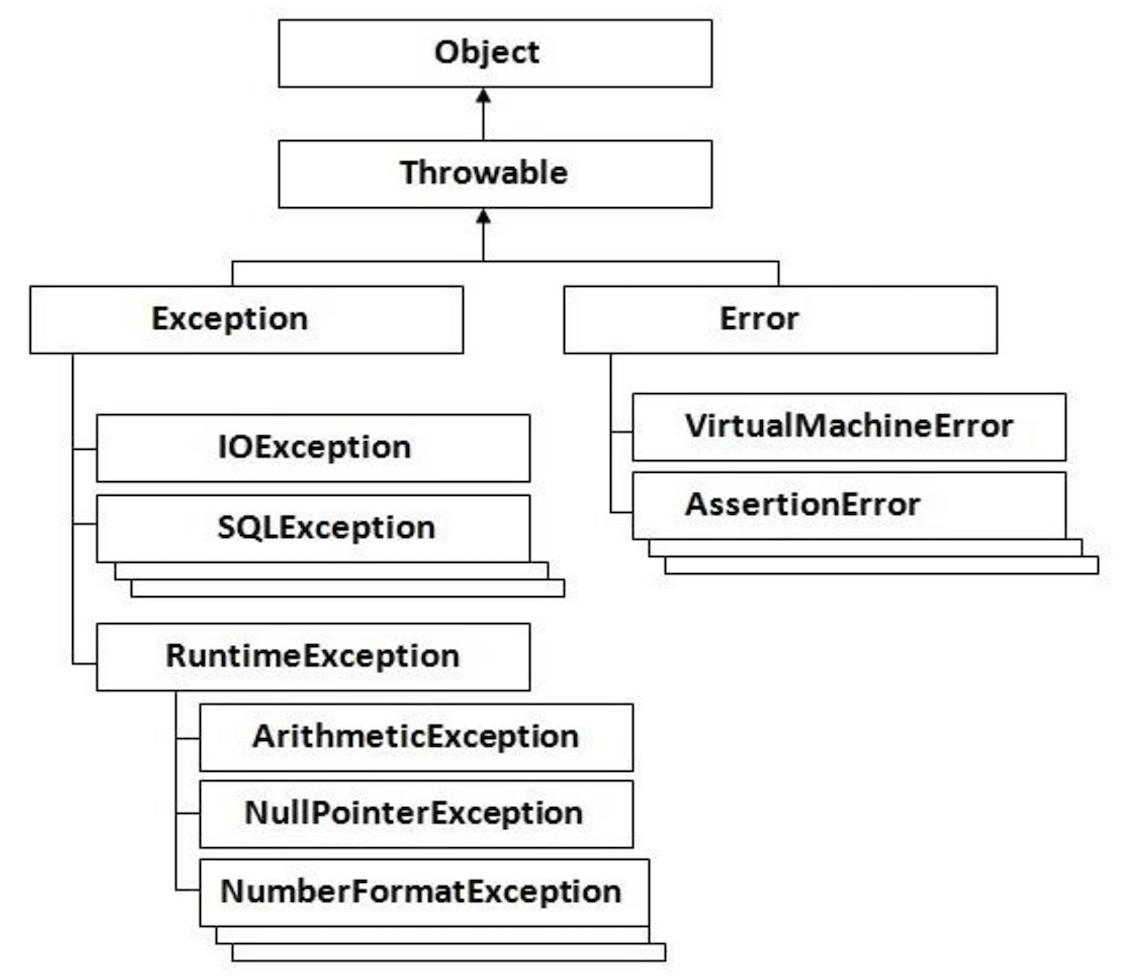
\includegraphics[scale=0.45]{rozdziały/images/PO/exceptions hierarchy.png}
\end{center}

Klasa \textit{Throwable} zawiera takie metody, jak na przykład \textit{getMessage()}, \textit{printStackTrace()} czy \textit{getCause()}, które przekazują więcej informacji o wyjątku.

Klasa \textit{Error} dotyczy poważnych problemów, które nie są przechwytywane. 

Klasa \textit{Exception} zawiera natomiast wyjątki (oprócz \textit{RuntimeException}), które powinny być obsługiwane przez program i są to tak zwane \textbf{wyjątki nadzorowane} (ang. \textit{checked exceptions}). \textbf{Wyjątki nienadzorowane} (ang. \textit{unchecked exceptions}) są to natomiast podklasy \textit{RuntimeException} i ich nie obsługujemy.

\subsection{Zgłaszanie wyjątków}

Zgłaszanie wyjątków odbywa się za pomocą słowa kluczowego \javainline{throw}, który przerywa normalne wykonanie programu. Następnie na stosie wykonania programu odbywa się poszukiwanie obsługi wyjątku: bloki i metody niezawierające obsługi są zdejmowane ze stosu, a brak obsługi kończy się przerwaniem działania programu.

Lista zgłaszanych przez metodę wyjątków jest deklarowana w jej nagłówku za pomocą \javainline{throws}. Lista ta zawiera tylko wyjątki nadzorowane oraz \purple{musi zawierać wszystkie zgłaszane przez metodę wyjątki} (choć może mieć też ich więcej). Podczas kompilacji kompilator weryfikuje poprawność tej listy.

Przy nadpisywaniu metody zakres tej listy \purple{może być węższy} niż metody nadrzędnej (ale \purple{nie może być szerszy}). Jest to ważne, by uniknąć sytuacji, w której nie możemy użyć obiektu podklasy jako obiektu nadklasy (ang. \textit{Liskov substitution}). Z tego powodu nie możemy zadeklarować więcej wyjątków niż było ich w nadklasie. Możemy zadeklarować mniej, ponieważ nadpisywana metoda, różniąca się od oryginalnej, mogłaby po prostu w kodzie wcale tych wyjątków nie rzucać, wtedy nie ma potrzeby deklarować ich w nagłówku. W przeciwnym wypadku bylibyśmy zmuszeni obsługiwać nierzucane wyjątki, używając obiektu danej klasy wprost (nie jako obiekt nadklasy), co byłoby bardzo niepraktyczne.

\subsection{Obsługa wyjątków}

Obsługa wyjątków odbywa się za pomocą instrukcji \javainline{try ... catch ...}. Po \javainline{try} wpisujemy normalne działanie algorytmu, w którym może wystąpić wyjątek, a po \javainline{catch} obsługę konkretnego wyjątku (instrukcji \javainline{catch} może być wiele i ich \purple{kolejność ma znaczenie}: jeśli kilka klauzul pasuje, to zostanie wybrana pierwsza z nich). W \javainline{catch} możemy też zgłosić wyjątek, ale nie będzie on już obsłużony w tej samej instrukcji \javainline{try ... catch ...}.

Do instrukcji \javainline{try ... catch ...} możemy jeszcze dodać dodatkową instrukcję \javainline{finally ...}, która zostanie wykonana zawsze przy wychodzeniu z bloku \javainline{try ... catch ...} (można też pominąć wszystkie \javainline{catch} i mieć tylko blok \javainline{try ... finally ...}). Instrukcje zawarte po \javainline{finally} wykonane zostaną zawsze, gdy złapany zostanie wyjątek (nawet taki niepasujący do żadnego \javainline{catch}).

\begin{example}
    W poniższym kodzie zaprezentowano obsługę wyjątków:
    \begin{java}
        public class UczymySieWyjatkow {
            void rzucamyWyjatkiem(String s) throws Exception1, Exception2 {
                System.out.println("Przed rzuceniem wyjątku");
                if (s == null) 
                    throw new Exception1();
                else if (s == "Rzucam studia")
                    throw new Exception2();
                System.out.println("Po rzuceniu wyjątku");
            }
    
            void obslugujemyWyjatek(String s) {
                try {
                    System.out.println("Przed wywołaniem niebezpiecznej funkcji");
                    rzucamyWyjatkiem(s);
                    System.out.println("Po wywołaniu niebezpiecznej funkcji");
                    
                // W jednej klauzuli catch można przechwycić kilka wyjątków
                } catch (Exception1 || Exception2 e) {
                    System.out.println("Obsługujemy wyjątek");
                    e.printStackTrace(System.out);
                } finally {
                    System.out.println("To wykonuje się zawsze");
                }
            }
    
            public static void main(String[] args) {
                UczymySieWyjatkow u = new UczymySieWyjatkow();
                System.out.println("Oby się udało");
                u.obslugujemyWyjatek(null);
                System.out.println("Udało się!");
            }
        }
    \end{java}

    Wykonanie takiego programu wypisze na wyjście:
    \begin{java}
        Oby się udało
        Przed wywołaniem niebezpiecznej funkcji
        Przed rzuceniem wyjątku
        Obsługujemy wyjątek
        java.lang.Exception1
            at test.UczymySieWyjatkow.rzucamyWyjatkiem(UczymySieWyjatkow.java:5) 
            at test.UczymySieWyjatkow.obslugujemyWyjatek(UczymySieWyjatkow.java:14) 
            at test.UczymySieWyjatkow.main(UczymySieWyjatkow.java:28)
        To wykonuje się zawsze
        Udało się!
    \end{java}
\end{example}

\subsection{Własne klasy wyjątków}

Możemy też definiować własne klasy wyjątków, są to podklasy \textit{Exception} lub \textit{RuntimeException}. Mogą zawierać dodatkowe pola i \purple{koniecznie muszą mieć konstruktor}. Standardowe klasy wyjątków mają przeważnie konstruktor przyjmujący napis (który można potem uzyskać na przykład metodą \textit{getMesssage()}). We własnych wyjątkach taki napis ustawiamy w konstruktorze za pomocą słowa kluczowego \javainline{super}.

\begin{example}
    Poniżej przedstawiony jest przykład własnej klasy wyjątku \textit{StudentRzucilStudia} oraz jego użycie:
    \begin{java}
        class StudentRzucilStudia extends Exception {
            StudentRzucilStudia(String s) {
                super(s);
            }
        }
    
        public class Student {
            public static void main(String[] args) {
                try {
                    throw new StudentRzucilStudia("Student debil");
                } catch (StudentRzucilStudia e) {
                    System.out.println(e.getMessage());
                }
            }
        }
    \end{java}
\end{example}

\begin{problems}
    \prob Dany jest program w języku Java:
    \begin{java}
        final class A {
        
            public boolean f(Object x) {
                return equals(x);
            }
            
            public boolean g(Object x) {
                return x.equals(this);
            }
        }
    \end{java}
    W takim programie
    \answers
    {wywołanie funkcji $f$ może zwrócić wyjątek klasy dziedziczącej po klasie \textit{Exception}}
    {wywołanie funkcji $f$ zawsze zwraca \textbf{false}}
    {wywołanie funkcji $g$ może zwrócić wyjątek klasy dziedziczącej po klasie \textit{Exception}}
    % {NIE}{NIE}{TAK}

    \prob Rozważamy programy napisane w języku Java. Jeżeli klasa $A$ jest nadklasą $B$, to 
    \answers
    {w treści klasy $B$ można zdefiniować metodę o takim samym nagłówku jak metoda zdefiniowana w klasie $A$}
    {jeśli obie klasy $A$ i $B$ mają po jednym konstruktorze, to w nagłówku konstruktora z klasy $B$ należy podać listę wyjątków obejmującą wszystkie wyjątki nadzorowane wymienione w~konstruktorze z klasy $A$}
    {w treści klasy $B$ można zdefiniować metodę o takim samym nagłówku jak metoda zdefiniowana w klasie $A$, ale z węższą widocznością niż była podana w metodzie z klasy $A$}
    % {TAK?}{TAK?}{NIE?}

    \prob W języku Java
    \answers
    {nie trzeba obsługiwać wszystkich wyjątków kontrolowanych (ang. \textit{checked exceptions})}
    {w podklasie można nadpisać (ang. \textit{override}) metodę i zadeklarować ją z węższą listą wyjątków}
    {implementując interfejs, w którym pewna metoda rzuca listą wyjątków, trzeba zadeklarować tę metodę z tymi wszystkimi wyjątkami (tj. lista rzucanych wyjątków (\texttt{throws}) jest dokładnie taka sama)}
    % {NIE}{TAK}{NIE}
\end{problems}

\section{Standardowe kolekcje w Javie}

\textbf{Kolekcja} to obiekt:
\begin{itemize}
    \item służący do przechowywania (innych) obiektów,
    \item udostępniający mechanizmy pozwalające na wstawianie, przeglądanie i pobieranie przechowywanych obiektów,
    \item nie mający zadanego specyficznego dla siebie rozmiaru.
\end{itemize}

\subsection{Hierarchia dziedziczenia}
Kolekcje w standardowej bibliotece Javy implementują różne interfejsy. Poniższy diagram pokazuje hierarchię dziedziczenia interfejsów, klasy abstrakcyjne oraz klasy kolekcji dostępnych w Javie.

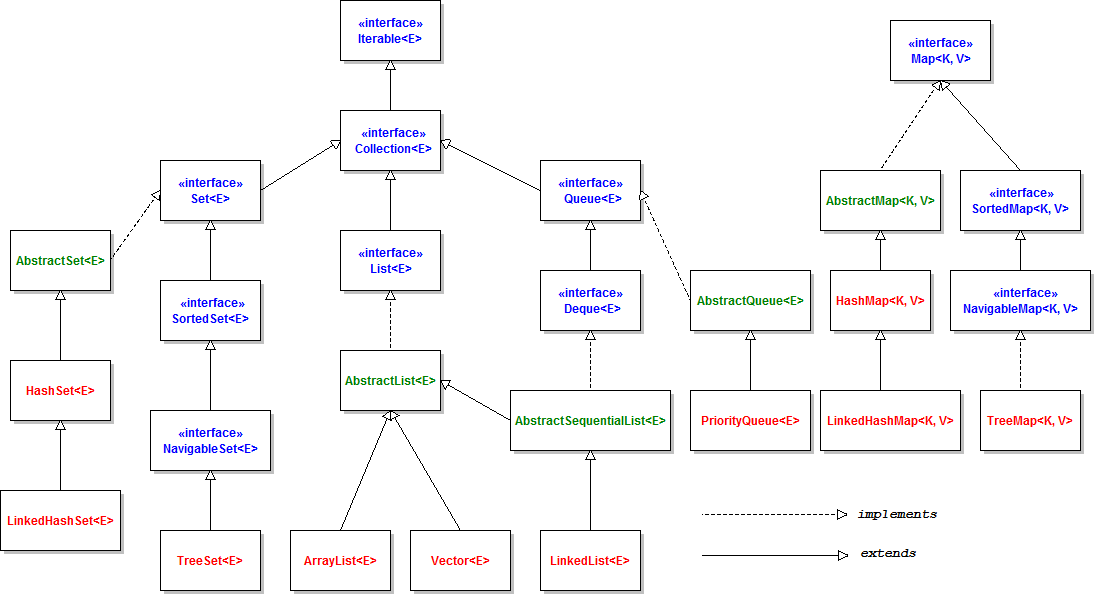
\includegraphics[scale=0.55]{rozdziały/images/PO/collections framework overview.png}

Warto zwrócić uwagę: klasy i interfejsy powyżej są generyczne (uogólnione), tzn. kolekcja może być dowolnego typu (\javainline{<E>}).

\subsection{Najważniejsze metody dostępne w interfejsie kolekcji}

\begin{java}
    // Dodaje element do kolekcji (operacja opcjonalna)
    boolean add(E e); 
    
    // Dodaje wszystkie elementy z danej kolekcji (operacja opcjonalna)
    boolean addAll(Collection<? extends E> c);  

    // Usuwa wszystkie elementy z tej kolekcji (operacja opcjonalna)
    void clear(); 
    
    // Zwraca true, jeśli ta kolekcja zawiera określony element
    boolean contains(Object o); 

    // Zwraca true, jeśli ta kolekcja zawiera wszystkie elementy z określonej kolekcji
    boolean containsAll(Collection<?> c); 

    // Porównuje określony obiekt z tą kolekcją pod kątem równości
    boolean equals(Object o); 

    // Zwraca true, jeśli ta kolekcja nie zawiera żadnych elementów
    boolean isEmpty(); 

    // Zwraca iterator po elementach w tej kolekcji
    Iterator<E> iterator(); 

    // Usuwa pojedynczy egzemplarz danego elementu, jeśli istnieje (operacja opcjonalna)
    boolean remove(Object o); 

    // Usuwa wszystkie elementy, które są zawarte w danej kolekcji (operacja opcjonalna)
    boolean removeAll(Collection<?> c); 

    // Zwraca liczbę elementów w kolekcji
    int size(); 
\end{java}

\begin{solutions}
    % Kasia K
    \sol Mówimy, że widoczność $A$ jest szersza niż widoczność $B$, gdy zawsze kiedy widoczne jest $B$, widoczne jest też $A$. Widoczność pakietowa jest szersza niż widoczność
    \answerss
    {publiczna}
    {chroniona}
    {prywatna}
    {NIE}{NIE}{TAK}

    Oznaczmy $A \succ B$, jeżeli widoczność $A$ jest szersza niż widoczność $B$. Z definicji zakresów widoczności wiemy, że zachodzi: publiczna $\succ$ chroniona $\succ$ pakietowa $\succ$ prywatna. Z tego natomiast bezpośrednio wynikają odpowiedzi.
    
    % tomasz G    
    \sol Dany jest kod w języku Java:
    \begin{java}
        class A {
            private int i1;
            protected int i2;
        }
        
        class B extends A {
            private int j1;
            
            public void m(B b) {
                // b.i1 = 0;
                // b.i2 = 0;
                // b.j1 = 0;
            }
        }    
    \end{java}
    Kod skompiluje się bez błędów po odkomentowaniu linii
    \answerss
    {\javainline{b.i1 = 0;}}
    {\javainline{b.i2 = 0;}}
    {\javainline{b.j1 = 0;}}
    {NIE}{TAK}{TAK}
    \begin{enumerate}[\bf A.]
        \item Ponieważ pole i1 jest \textbf{prywatnym} polem klasy A, nie jest ono dostępne w klasie B.

        \item pole i2 ma widoczność \textbf{protected}, czyli jest dostępne również w klasach dzedziczących.

        \item pole j1 jest polem \textbf{prywatnym}, ale w klasie B, czyli tej w której aktualnie się znajdujemy.
    \end{enumerate}


    % Michał
    \sol Dana jest definicja klasy w języku Java:
    \begin{java}
        final class A {
            static A a;
            A() { a = this; }
            static boolean f() { return a.equals(a); }
            boolean g() { return a == this; }
            boolean h() { return equals(this); }
        }
    \end{java}
    Dla takiej klasy
    \answerss
    {każde wywołanie funkcji $f$ daje wynik \textbf{true}}
    {każde wywołanie funkcji $g$ daje wynik \textbf{true}}
    {każde wywołanie funkcji $h$ daje wynik \textbf{true}}
    {NIE}{NIE}{TAK}

    \begin{enumerate}[\bf A.]
        \item Funkcja $f$ jest statyczna, zatem można ją wywołać bez wywoływania konstruktora $A$. W takim przypadku $a$ będzie {\ttfamily NULL}-em i wywołanie funkcji zakończy się błędem.

        \item Operator \javainline{==} porównuje adresy, które tutaj nie muszą być równe.

        \item Domyślna implementacja \javainline{equals()} porównuje adresy, a jako że porównujemy obiekt z samym sobą to zawsze otrzymamy \textbf{true}.
    \end{enumerate}

    % Patryk
    \sol Dany jest program w języku Java:
    \begin{java}
        class A {
            public void m1() { System.out.println("A"); }
            public void m2(A a) { a.m1(); }
        }
        
        class B extends A {
            public void m1() { System.out.println("B"); }
        }
        
        class C extends B {
            public void m1() { System.out.println("C"); }
            public void m2(A a) { a.m2(this); }
        }
        
        public class Test {
            public static void main(String[] args) {
                A a1 = new A();
                A a2 = new B();
                A a3 = new C();
                a3.m1();   // (a)
                a2.m2(a3); // (b)
                a3.m2(a1); // (c)
            }
        }
    \end{java}
    Podczas wykonania
    \answerss
    {wiersza \javainline{a3.m1();} tego programu zostanie wypisane \texttt{A}}
    {wiersza \javainline{a2.m2(a3);} tego programu zostanie wypisane \texttt{B}}
    {wiersza \javainline{a3.m2(a1);} tego programu zostanie wypisane \texttt{C}}
    {NIE}{NIE}{TAK}

    \begin{enumerate}[\bf A.]
        \item Zgodnie z typem faktycznym (a nie zadeklarowanym) obiektu \textit{a3}, wywoła się metoda \textit{m1()} zdefiniowana w klasie \textit{C}, więc wypisane zostanie \texttt{C}.
        
        \item Wywoła się metoda \textit{m2()} zdefiniowana w klasie \textit{A} z argumentem klasy \textit{C}, więc wywołanie \textit{a.m1()} spowoduje wypisanie się \texttt{C}.

        \item Wywoła się metoda \textit{m2()} zdefiniowana w klasie \textit{C} z argumentem klasy \textit{A}. Następnie \textit{a.m2()} spowoduje wywołanie się metody z klasy \textit{A} z argumentem klasy \textit{C}. To spowoduje wywołanie się metody \textit{m1()} z klasy \textit{C}, więc zostanie wypisane \texttt{C}.
    \end{enumerate}

    % Patryk
    \sol Rozważamy programy napisane w języku Java. Jeżeli klasa $A$ jest nadklasą $B$, to w treści klasy $B$
    \answerss
    {trzeba zdefiniować wszystkie metody zdefiniowane w klasie $A$}
    {można zdefiniować metody o innych nagłówkach niż metody zdefiniowane w klasie $A$}
    {można zdefiniować metodę o takim samym nagłówku jak metoda zdefiniowana w klasie $A$, ale z węższą widocznością niż była podana w metodzie z klasy $A$}
    {NIE}{TAK}{NIE/TAK}

    \begin{enumerate}[\bf A.]
        \item Nie trzeba, część metod może być zaimplementowana w klasie \textit{A} lub klasa \textit{B} może być klasą abstrakcyjną.

        \item Jak najbardziej można utworzyć własne metody, niezdefiniowane w \textit{A}.

        \item Jeżeli autor miał na myśli nadpisanie funkcji, to nie, bo takie można dać jedynie z takim samym nagłówkiem i szerszą widocznością.\\
        W ogólności klasy A i B mogą należeć do innych pakietów i wtedy jeżeli funkcja w A ma widoczność pakietową, to odpowiednia funkcja zdefiniowana w B może być prywatna, więc odpowiedź to tak.
        
    \end{enumerate}

    % Błażej
    \sol Dany jest program w języku Java:
    \begin{java}
        class A {
            public A() { System.out.print("1"); m1(); }
            public A(int i) { System.out.print("2"); }
            public A(A a) { System.out.print("3"); }
            public void m1() { System.out.print("4"); }
        }

        class B extends A {
            A a;
            public B(A a) { System.out.print("5"); }
            public B() { this(new A(0)); System.out.print("6"); }
            @Override
            public void m1() { System.out.print("7"); }
        }

        public class Main {
            public static void main(String[] args) {
                A a = new B();
            }
        }
    \end{java}
    Po uruchomieniu tego programu na pewno (oprócz, być może, innych znaków) zostanie wypisana cyfra
    \answerss
    {1}
    {4}
    {3}
    {TAK}{NIE}{NIE}

    Prześledźmy wykonanie kodu krok po kroku:
    \begin{itemize}
        \item Tworzony jest obiekt klasy \textit{B} poprzez wywołanie jego bezargumentowego konstruktora.
        
        \item Wywołanie \javainline{this(new A(0))} powoduje utworzenie obiektu \textit{A} z użyciem konstruktora \javainline{A(int i)} -- wypisana zostanie ,,2''.

        \item Następnie wywołujemy konstruktor \javainline{B(A a)}. Ponieważ klasa \textit{B} dziedziczy po \textit{A}, a pierwszą linijką konstruktora nie jest wywołanie konstruktora nadklasy, to automatycznie wywołany zostanie konstruktor bezargumentowy klasy \textit{A} -- wypisana zostanie ,,1''

        \item Konstruktor bezargumentowy klasy \textit{A} wywoła metodę \textit{m1} obiektu \textit{B}, który tę metodę nadpisał -- wypisana zostanie ,,7''.

        \item Dalej, konstruktor \javainline{B(A a)} wypisze ,,5''.

        \item Ostatecznie, konstruktor bezargumentowy klasy \textit{B} wypisze ,,6'', co zakończy działanie programu.
    \end{itemize}

    Warto zwrócić uwagę na to, że gdyby w funkcji \textit{main()} zamienić deklarację typu obiektu z klasy \textit{A} na \textit{B} (tj. \javainline{B b = new B();}), nie zmieniłoby to przebiegu wykonania programu.

    % Grześ
    \sol Dany jest program w języku Java:
    \begin{java}
        class A {
          void m1() { System.out.println("1"); }
          static void m2() { System.out.println("2"); }
          void m3() { m1(); }
          void m4() { m2(); }
        }
        
        class B extends A {
          @Override
          void m1( ) { System.out.println("3"); }
          static void m2() { System.out.println("4"); }
        }
    
        public class Main {
          public static void main(String[] args) {
            A a = new B();
            a.m1();
            a.m3();
            a.m4();
          }
        }    
    \end{java}
    W takim programie
    \answerss
    {wywołanie \javainline{a.m1()} spowoduje wypisanie jedynki}
    {wywołanie \javainline{a.m3()} spowoduje wypisanie jedynki}
    {wywołanie \javainline{a.m4()} spowoduje wypisanie dwójki}
    {NIE}{NIE}{TAK}
    Obiekt \texttt{a} jest typu \texttt{A}, ale do jego stworzenia użyto konstruktora klasy \texttt{B}, więc metody zostały odziedziczone.
    
    \textbf{A.} Metoda \texttt{m1()} została nadpisana przez podklasę \texttt{B}, więc zostanie wypisane 3.

    \textbf{B.} Metoda \texttt{m3()} wywołuje metodę \texttt{m1()}, która została nadpisana przez podklasę \texttt{B}, więc zostanie wypisane 3.

    \textbf{C} Metoda \texttt{m2()} jest statyczna, czyli została ona statycznie powiązana z typem obiektu \texttt{a} podczas kompilacji. Znaczy to, że wypisane zostanie 2.

    % Tutaj wyjaśnienie od chatu gpt:
    
    % Here's the breakdown of the output:

    % \begin{enumerate}
    % \item \texttt{A a = new B();} creates a new object \texttt{a} of type \texttt{A} but referencing an instance of class \texttt{B}. Polymorphism allows the overridden methods to be called from the subclass.
    % \item \texttt{a.m1();} invokes the \texttt{m1()} method. Since \texttt{a} is referencing an instance of class \texttt{B}, the overridden method in class \texttt{B} will be called, resulting in the output "3".
    % \item \texttt{a.m3();} invokes the \texttt{m3()} method. This method calls \texttt{m1()}. Again, since \texttt{a} is referencing an instance of class \texttt{B}, the overridden method in class \texttt{B} will be called, resulting in the output "3".
    % \item \texttt{a.m4();} invokes the \texttt{m4()} method. This method calls \texttt{m2()}. However, since \texttt{m2()} is a static method, it is resolved at compile-time based on the reference type (\texttt{A}). Therefore, the output will be "2".
    % \end{enumerate}

    % Julia
    \sol Dany jest program w języku Java:
    \begin{java}
        final class A {
        
            public boolean f(Object x) {
                return equals(x);
            }
            
            public boolean g(Object x) {
                return x.equals(this);
            }
        }
    \end{java}
    W takim programie
    \answerss
    {wywołanie funkcji $f$ może zwrócić wyjątek klasy dziedziczącej po klasie \textit{Exception}}
    {wywołanie funkcji $f$ zawsze zwraca \textbf{false}}
    {wywołanie funkcji $g$ może zwrócić wyjątek klasy dziedziczącej po klasie \textit{Exception}}
    {NIE}{NIE}{TAK}

    \begin{enumerate}[\bf A.]
        \item Nie, ponieważ wykona się funkcja \textit{equals()} na obiekcie klasy \textit{A}. Funkcja ta jest domyślnie zdefiniowana i nie rzuca wyjątkiem podklasy \textit{Exception}.

        \item Może zwrócić \textbf{true}, na przykład gdy obiektem \textit{x} będzie \javainline{this}. Wtedy zostanie wykonane porównanie \javainline{this.equals(this)}, które zwraca \textbf{true}.

        \item Jeżeli obiekt \textit{x} będzie równy \texttt{NULL}, to dostaniemy \textit{NullPointerException}, który jest podklasą klasy \textit{RuntimeException}, zatem też i \textit{Exception}.
    \end{enumerate}

    \sol Rozważamy programy napisane w języku Java. Jeżeli klasa $A$ jest nadklasą $B$, to 
    \answerss
    {w treści klasy $B$ można zdefiniować metodę o takim samym nagłówku jak metoda zdefiniowana w klasie $A$}
    {jeśli obie klasy $A$ i $B$ mają po jednym konstruktorze, to w nagłówku konstruktora z klasy $B$ należy podać listę wyjątków obejmującą wszystkie wyjątki nadzorowane wymienione w~konstruktorze z klasy $A$}
    {w treści klasy $B$ można zdefiniować metodę o takim samym nagłówku jak metoda zdefiniowana w klasie $A$, ale z węższą widocznością niż była podana w metodzie z klasy $A$}
    {TAK}{TAK}{NIE/TAK}

    \begin{enumerate}[\bf A.]
        \item Można, zostanie ona wtedy nadpisana (jeśli nie jest to metoda prywatna) lub zdefiniowana jako nowa (jeśli jest prywatna).

        \item Ponieważ konstruktor podklasy zawiera wywołanie konstruktora nadklasy (jeśli nie jest ono jawne, kompilator sam ,,doda'' jego wywołanie), konstruktor podklasy musi deklarować te same wyjątki, co konstruktor nadklasy.

        \item Patrz zadanie 5.
    \end{enumerate}

    % Filip
    \sol W języku Java
    \answerss
    {nie trzeba obsługiwać wszystkich wyjątków kontrolowanych (ang. \textit{checked exceptions})}
    {w podklasie można nadpisać (ang. \textit{override}) metodę i zadeklarować ją z węższą listą wyjątków}
    {implementując interfejs, w którym pewna metoda rzuca listą wyjątków, trzeba zadeklarować tę metodę z tymi wszystkimi wyjątkami (tj. lista rzucanych wyjątków (\texttt{throws}) jest dokładnie taka sama)}
    {NIE}{TAK}{NIE}

    \begin{enumerate}[\bf A.]
        \item Deklarowanie wyjątku jako wyjątek kontrolowany zobowiązuje nas do obsłużenia go w jakiś sposób -- po to go w ogóle tak piszemy.

        \item Możemy tak zrobić -- jedyne co jest ważne to to, żeby ta lista wyjątków była kompatybilna z listą metody z nadklasy, żeby nie było sytuacji, w której nie możemy użyć obiektu podklasy jako obiektu nadklasy (ang. \textit{Liskov substitution}). Z tego powodu nie możemy zadeklarować więcej wyjątków niż było w nadklasie. Możemy zadeklarować mniej, ponieważ nadpisywana metoda, różniąca się od oryginalnej, mogłaby po prostu w kodzie wcale tych wyjątków nie rzucać, wtedy nie ma potrzeby deklarować ich w nagłówku. W przeciwnym wypadku bylibyśmy zmuszeni obsługiwać nierzucane wyjątki, używając obiektu danej klasy wprost (nie jako obiekt nadklasy), co byłoby bardzo niepraktyczne.

        \item Nie, z tego samego powodu co powyżej. Z praktycznego/logicznego punktu widzenia -- nie miałoby sensu wymuszanie tej samej listy wyjątków, bo programista piszący metodę z implementowanego interfejsu wcale nie musiałby napisać kodu, który rzuca każdy wymieniony wyjątek.
    \end{enumerate}
\end{solutions}